\documentclass[aps,letterpaper,10pt]{revtex4}
\input kvmacros % For Karnaugh Maps (K-Maps)

\usepackage{graphicx} % For images
\usepackage{float}    % For tables and other floats
\usepackage{verbatim} % For comments and other
\usepackage{amsmath}  % For math
\usepackage{amssymb}  % For more math
\usepackage{fullpage} % Set margins and place page numbers at bottom center
\usepackage{listings} % For source code
\usepackage{subfig}   % For subfigures
\usepackage[usenames,dvipsnames]{color} % For colors and names
\usepackage[pdftex]{hyperref}           % For hyperlinks and indexing the PDF
\hypersetup{ % play with the different link colors here
    colorlinks,
    citecolor=blue,
    filecolor=blue,
    linkcolor=blue,
    urlcolor=blue % set to black to prevent printing blue links
}

\definecolor{mygrey}{gray}{.96} % Light Grey
\lstset{ 
	language=[ISO]C++,              % choose the language of the code ("language=Verilog" is popular as well)
   tabsize=4,							  % sets the size of the tabs in spaces (1 Tab is replaced with 3 spaces)
	basicstyle=\tiny,               % the size of the fonts that are used for the code
	numbers=left,                   % where to put the line-numbers
	numberstyle=\tiny,              % the size of the fonts that are used for the line-numbers
	stepnumber=2,                   % the step between two line-numbers. If it's 1 each line will be numbered
	numbersep=5pt,                  % how far the line-numbers are from the code
	backgroundcolor=\color{mygrey}, % choose the background color. You must add \usepackage{color}
	%showspaces=false,              % show spaces adding particular underscores
	%showstringspaces=false,        % underline spaces within strings
	%showtabs=false,                % show tabs within strings adding particular underscores
	frame=single,	                 % adds a frame around the code
	tabsize=3,	                    % sets default tabsize to 2 spaces
	captionpos=b,                   % sets the caption-position to bottom
	breaklines=true,                % sets automatic line breaking
	breakatwhitespace=false,        % sets if automatic breaks should only happen at whitespace
	%escapeinside={\%*}{*)},        % if you want to add a comment within your code
	commentstyle=\color{BrickRed}   % sets the comment style
}

% Make units a little nicer looking and faster to type
\newcommand{\Hz}{\textsl{Hz}}
\newcommand{\KHz}{\textsl{KHz}}
\newcommand{\MHz}{\textsl{MHz}}
\newcommand{\GHz}{\textsl{GHz}}
\newcommand{\ns}{\textsl{ns}}
\newcommand{\ms}{\textsl{ms}}
\newcommand{\s}{\textsl{s}}



% TITLE PAGE CONTENT %%%%%%%%%%%%%%%%%%%%%%%%
% Remember to fill this section out for each
% lab write-up.
%%%%%%%%%%%%%%%%%%%%%%%%%%%%%%%%%%%%%%%%%%%%%
\newcommand{\labtitle}{Numpy, get rid of the Mathesaurus}
\newcommand{\authorname}{Alessandro Ferrari}
\newcommand{\emailauthor}{alessandroferrari87@gmail.com}
\newcommand{\classno}{Remote Sensing}
\newcommand{\professor}{Prof. Alberto Signoroni}
\newcommand{\university}{Universit\'a degli Studi di Brescia}
\newcommand{\presentationdate}{27 November 2013, Brescia}
% END TITLE PAGE CONTENT %%%%%%%%%%%%%%%%%%%%


\begin{document}  % START THE DOCUMENT!


% TITLE PAGE %%%%%%%%%%%%%%%%%%%%%%%%%%%%%%%%%%%%%%
% If you'd like to change the content of this,
% do it in the "TITLE PAGE CONTENT" directly above
% this message
%%%%%%%%%%%%%%%%%%%%%%%%%%%%%%%%%%%%%%%%%%%%%%%%%%%

\begin{titlepage}
\begin{center}
{\Large \textsc{\labtitle} \\ \vspace{4pt}} 
\rule[13pt]{\textwidth}{1pt} \\ \vspace{150pt}
{\large author: \authorname \\ \vspace{10pt}
email: \emailauthor \\ \vspace{10pt}}
\end{center}
\end{titlepage}
% END TITLE PAGE %%%%%%%%%%%%%%%%%%%%%%%%%%%%%%%%%%

%%%%%%%%%%%%%%%%%%%%%%%%%%%%%%
%%%%%%%%%%%%%%%%%%%%%%%%%%%%%%
\section{Introduction}
Many of us are scientists or former scientists. Any kind of scientist you are or you will be, you will need to develop, at least, basic data scientists skills. You will need to effectively read, handle, manipulate and visualize data for your professional activities, either you want to monitor vibrations of a mechanical component or to show trends of an advertising campaign of the company that you work for. In order to do so, nobody of us wants to re-invent the wheel, luckily there are easy to use and efficiently written software libraries that provides us the basic bricks for analysing our data.\vspace{3mm}

Many of you are probably more acquainted with technologies for data analysis such as Matlab. Numpy and Python frameworks are definitely not just the cheaper alternative to the Matlab environment. While offering an outstanding variety of different scientific tools, that beats competitors in many different applications, \textit{i.e.} image analysis or machine learning, they mantain the same easiness for prototyping as Matlab, but freeing the user to the burden of a heavy development environment (the Mathesaurus).\vspace{3mm} 

Python is a language created by hackers for hackers, its power is comparable to its easiness. By developing solutions with it, you can create solution that are ready to go to market in the same time that you were spending while doing your prototypes. What are you waiting for? Join the makers movement! \vspace{3mm}  
 
This lab will guide you step by step through the use of numpy to manipulate scientific data, and matplotlib to visualize them. \vspace{3mm}

%%%%%%%%%%%%%%%%%%%%%%%%%%%%%%
\section{Instruction to the use of this lab}
By this lab, you can learn many precious stuffs that can make the difference in your professional career as a technology professional. When you do things actively you can memorize also ten times more, so make yourself a gift, be active! There are few rules that you need to follow:
\begin{itemize}
\item Do you have numpy documentation website open? If you do not, I will not help you.
\item Did your lab mate ask you a question without having opened the numpy website documentation? Do not help him.
\item Are you having troubles on finding numpy documentation online? Click  \href{http://lmgtfy.com/?q=numpy+doc}{here}.
\item{You will find the code of the guided track in the folder of the lab, so you can avoid to spend time while copy/pasting functions. Try to understand the different topics and then get involved in the exercises so that you can learn how to apply what you have learnt.}
\item{Be active.}
\item{Enjoy!}
\item{Please, send me feedback to improve the laboratory for next years.}
\end{itemize}
Are you ready? Let's go!

%%%%%%%%%%%%%%%%%%%%%%%%%%%%%%%
\section{Numpy and matplotlib}
\subsection{Array objects}
NumPy provides an N-dimensional array type, the \textit{ndarray}, which describes a collection of “items” of the same type. The items can be indexed using for example N integers.

All ndarrays are homogenous: every item takes up the same size block of memory, and all blocks are interpreted in exactly the same way. The type of the items in the array is specified by an attribute called \textit{dtype} that is in every \textit{ndarray}. Thus, ndarrays are not as python lists, that are heterogeneous, so that can contains items of different types.

An item extracted from an array, \textit{e.g.}, by indexing, is represented by a Python object whose type is one of the array scalar types built in Numpy. The array scalars allow easy manipulation of also more complicated arrangements of data.

First of all, you need to import the numpy module:
\begin{lstlisting}
import numpy as np
\end{lstlisting}
It is renamed as np for a convenient convention.

Then, you can create your array, by specifying its elements in a python list:
\begin{lstlisting}
#### NDARRAY CREATION ####
print "Create a 1D ndarray:"
a = np.array([0, 1, 2, 3])
print "a = %(a)s.\n" % {"a":a}
\end{lstlisting}
A numpy array can contain an audio signal, an image, an hyperspectral hypercube or any other kind of digital signal.
The ndarray object contains an attributes called \textit{ndim} that indicates the number of dimensions of the array, and an attribute \textit{shape} that contains the cardinality of the array in each dimension:
\begin{lstlisting}
### NDARRAY NUMBER OF DIMENSIONS AND SHAPE ###
print "Access to the ndim and shape attributes of a ndarray:"
print "a.ndim = %(ndim)s" % { "ndim" : a.ndim }
print "a.shape = %(shape)s" % { "shape" : a.shape }
print "len(a) = %(len)s.\n" % { "len" : len(a) } #len return the length of the first dimension
\end{lstlisting}
Note the syntax used for string formatting, it can be useful when you need to print more complicated strings.
For creating arrays biggers than 1 dimension, you can use the following syntax:
\begin{lstlisting}
### 2D NDARRAY ###
print "Creating a 2D ndarray:"
b = np.array([[0, 1, 2], [3, 4, 5]])    # 2 x 3 array
print "b = %(b)s" % {"b":b}
print "b.ndim = %(ndim)s" % {"ndim":b.ndim}
print "b.shape = %(shape)s" % {"shape":b.shape}
print "len(b) = %(len)s.\n" % {"len":len(b)}

### 3D NDARRAY ###
print "Creating a 3D ndarray:"
c = np.array([[[1], [2]], [[3], [4]]])    # 2 x 2 x 1 array
print "c = %(c)s" % {"c":c}
print "c.ndim = %(ndim)s" % {"ndim":c.ndim}
print "c.shape = %(shape)s" % {"shape":c.shape}
print "len(c) = %(len)s.\n" % {"len":len(c)}
\end{lstlisting}
What about create a 5D array? Try on your own!

To enter the items of the array one by one is rather unpractical in many cases. Some functions to generate numpy arrays without specifying the items will be introduced.
The function \textit{arange} creates a numpy array containing a sequence of evenly spaced items. The number of items is specified as a parameter. By default, the starting item of the sequence is 0 and the step between each item is 1.
\begin{lstlisting}
### NDARRAY WITH np.arange ### 
print "Construct a ndarray with np.arange:"
a = np.arange(10)
print "np.arange(10) = %{a}s" % {"a":a} 
\end{lstlisting}
What about if you want a sequence that do not start from 0 and has step different than 1?
\begin{lstlisting}
### NDARRAY WITH np.arange WITH MORE PARAMETERS ###
print "Use np.arange with more parameters:"
b = np.arange(1,9,2) # start = 1 ; end = 9 ; step = 2
print "np.arange(1,9,2) = %(b)s.\n" % {"b":b}
\end{lstlisting}
The function \textit{linspace} creates a numpy array containing a sequence with start, end and number of points in between specified as parameters. 
\begin{lstlisting}
### NDARRAY WITH np.linspace ###
print "Construct a ndarray with np.linspace:"
a = np.linspace(0,1,6) # start = 0 ; end = 1 ; number of points in between = 6
print "np.linspace(0,1,6) = %(linspace)s" % {"linspace":a}
print " ... and if you want to omit the endpoint in the sequence:"
b = np.linspace(0,1,6,endpoint=False)
print "np.linspace(0,1,6,endpoint=False) = %(linspace)s.\n" % {"linspace":b}
\end{lstlisting}
Then, there are some functions to create common arrays, such as the ones that you are familiar with in matlab. The function \textit{zeros} creates an array of 0 with size specified as a parameter, the function \text{ones} does the same, but with 1 instead of 0. The function \textit{eye} creates an identity matrix with diagonal of length specified as a parameter, while the function \textit{diag} creates a diagonal matrix with values of the items on the diagonal specified in a list passed in input as a parameter.
\begin{lstlisting}
### NDARRAY WITH np.zeros ###
print "Construct a ndarray with np.zeros:"
a = np.zeros( (3,3) )  #the size of the zeros array is specified with a tuple
print "np.zeros( (3,3) ) = %(zeros)s.\n" % {"zeros":a}

### NDARRAY WITH np.ones ###
print "Construct a ndarray with np.ones:"
b = np.ones( (3,3) )  #the size of the ones array is specified with a tuple
print "np.ones( (3,3) ) = %(ones)s.\n" % {"ones":b}

### NDARRAY WITH np.eye ###
print "Construct a ndarray with np.eye:"
c = np.eye(3)  #the number of ones in the diagonal in the identity matrix is specified as a parameter
print "np.eye(3) = %(eye)s.\n" % {"eye":c}

### NDARRAY WITH np.diag ###
print "Construct a ndarray with np.diag:"
d = np.diag([1,2,3,4]) #the items in the diagonal are specified as a list
print "np.diag([1,2,3,4]) = %(diag)s.\n" % {"diag":d}
\end{lstlisting}
When performing simulations, the creation of randomly generated arrays can be useful. The function \textit{seed} initialize the random numbers pseudo generator, if the seed is not specified, by default it is None and the pseudo random generator is initialized by looking at the system time. The function \textit{rand} generates a vector containing items distributed according a uniform probability distribution between 0 and 1. The function \textit{randn} generates a vector containing items distributed according a gaussian probability distribution.
\begin{lstlisting}
### INITIALIZE THE PSEUDO RANDOM NUMBER GENERATOR WITH np.random.seed ###
print "Initialize the pseudo random number generator with np.random.seed ..."
np.random.seed()

### RANDOM NDARRAY WITH np.random.rand ###
print "Construct a ndarray with np.rand:"
a = np.random.rand(4) #vector of 4 items chosen according to a U[0,1] prob. distribution
print "np.random.rand(4) = %(rand)s.\n" % {"rand":a}

### RANDOM NDARRAY WITH np.random.randn ###
print "Construct a ndarray with np.random.randn:"
b = np.random.randn(4) #vector of 4 items chosen according to gaussian dist., mean = 0, sigma = 1
print "np.random.randn(4) = %(randn)s.\n" % {"randn":b}
\end{lstlisting}
\subsection{Basic numpy data types}
Numpy arrays require uniformly typed items and they supports only certain defined types. In this subsection you will learn about the \textit{dtype} attribute of the ndarray and you will be introduced to the most common numpy data types.
\begin{lstlisting}
### dtype ATTRIBUTE IN ndarray ###
print "Check the type of the items by means of dtype attribute:"
a = np.array([0,1,2,3])
print "a.dtype of a = np.array([0,1,2,3]) is %(dtype)s." % {"dtype":a.dtype}
b = np.array([0.,1.,2.,3.])
print "b.dtype of b = np.array([0.,1.,2.,3.]) is %(dtype)s." % {"dtype":b.dtype}
print "You can also explicitely specify the type of the array that you are creating:"
c = np.array([0,1,2,3],dtype=float)
print "c.dtype of c = np.array([0,1,2,3],dtype=float) is %(dtype)s." % {"dtype":c.dtype}
print "The default data type is float:"
d = np.ones((3,3))
print "d.dtype of d = np.ones((3,3)) is %(dtype)s." % {"dtype":d.dtype}
print "Following some other types:"
e = np.array([1+2j, 3+4j, 5+6*1j])
print "e.dtype of e = np.array([1+2j, 3+4j, 5+6*1j]) is %(dtype)s." % {"dtype":e.dtype}
f = np.array([True, False, False, True])
print "f.dtype of f = np.array([True, False, False, True]) is %(dtype)s." % {"dtype":f.dtype}
g = np.array(['Bonjour', 'Hello', 'Hallo',])
print "g.dtype of g = np.array(['Bonjour', 'Hello', 'Hallo',]) is %(dtype)s." % {"dtype":g.dtype}
print "It is a string of maximum 7 characters!"
print "Some others useful types are int8, int16, int32, int64, uint8, uint16, uint32, uint34, float32 and many others. uint8 and float32 are especially useful if you use OpenCV library python bindings.\n"
\end{lstlisting}
\subsection{Visualizing data}
In this subsection, matplotlib will be briefly introduced. Matplotlib is probably the single most used Python package for 2D-graphics. It provides both a very quick way to visualize data from Python and publication-quality figures in many formats. Let me say that matplotlib is really a jewell for visualizing data, you will love it when you will start to get use to it. Furthermore, the potential of the library goes further beyond respect what it will be shown today. It has also some basic functions for 3d plotting, however if you want to plot 3d stuffs, you should evaluate more specialized modules as mayavi. Some examples of 1D plots (fig.1) follow:
\begin{lstlisting}
#IMPORT THE MATPLOTLIB MODULE
import matplotlib.pyplot as plt  # the tidy way

print "Basic usage of matplotlib for 1D plotting:"

#POPULATE THE X AND Y ARRAY FOR PLOTTING THE GRAPH
x = np.linspace(0, 3, 20)
y = np.linspace(0, 9, 20)

#1D LINE PLOT OF THE GRAPH
plt.plot(x, y)       # line plot 
plt.show()           # <-- shows the plot

#1D POINTS PLOT OF THE GRAPH
plt.plot(x, y, 'o')  # dot plot
plt.show()           # <-- shows the plot
\end{lstlisting}
\begin{figure}[h]
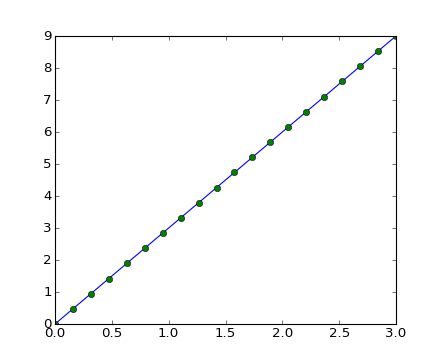
\includegraphics[scale=0.3]{img/numpy_plot1D.png}
\caption{Example of 1D plots.}\label{fig:1}
\end{figure}
An example of 2D plotting, in particular a function for showing images (fig.2), is shown in the code below:
\begin{lstlisting}
print "Basic usage of matplotlib for 2D plotting:"
image = np.random.rand(30, 30)
plt.imshow(image, cmap=plt.cm.hot)  
plt.colorbar()
plt.show()
\end{lstlisting}
\begin{figure}[h]
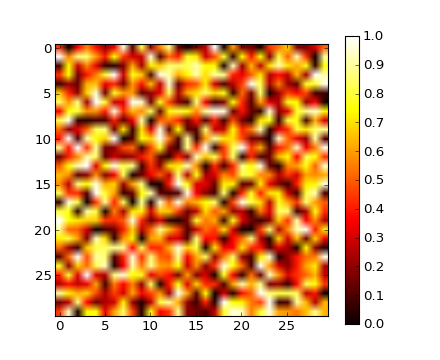
\includegraphics[scale=0.3]{img/numpy_plot2D.png}
\caption{Example of 2D plots.}\label{fig:2}
\end{figure}
These are just the most basic stuffs, however, in order to give you a glimpse of the stuffs that you can do with matplotlib, take a look to fig.3, that is possible to find at the end of the lab track.
\subsection{Indexing and Slicing}
Numpy arrays are zero-based (differently from Matlab array, that are 1 based). The items of an array can be accessed using indexing at the same way as other Python sequences (\textit{e.g.} lists):
\begin{lstlisting}
### INDEXING OF NUMPY ARRAYS ###
print "Indexing of numpy array's items:"
a = np.arange(10)
a_items = (a[0], a[3], a[-1]) #the index equals to -1 points to the last item
print "(a[0], a[3], a[-1]) = %(tuple)s where a = %(arange)s.\n" % {"tuple":a_items,"arange":a}
\end{lstlisting}
For multidimensional arrays, indexes are tuples of integers:
\begin{lstlisting}
### MULTIMENSIONAL INDEXING OF NUMPY ARRAYS ###
print "Multidimensional indexing of numpy array's items:"
a = np.diag(np.arange(3))
print "a[1, 1] = %(a11)s where a = %(a)s" % {"a11":a[1,1],"a":a}
print "Assigning of multidimensional numpy arrays:"
a[2,1]=10
print "if a[2,1] is assigned equal to 10, where a was %(a)s, then a = %(a_new)s.\n" % {"a":np.diag(np.arange(3)),"a_new":a}
\end{lstlisting}
Numpy arrays, like other Python sequences can also be sliced:
\begin{lstlisting}
### SLICING OF NUMPY ARRAYS ###
print "Slicing of numpy arrays:"
a = np.arange(10)
a_sliced = a[2:9:3] # [start:end:step]
print "a[2:9:3] = %(a_sliced)s where a = %(a)s. The order of the indices used to slice the array is relatively [start:end:step]. If the step index is omitted, by default is equal to 1." % {"a_sliced":a_sliced,"a":a}
a_sliced_2 = a[:4] # [0:end:1]
print "a[:4] = %(a_sliced_2)s where a = %(a)s. The start index is missing, so the slicing start by default from the index 0. Also the step index is missing, so by default the step is 1." % {"a_sliced_2":a_sliced_2,"a":a}
a_sliced_3 = a[1:3]
print "a[1:3] = %(a_sliced_3)s where a = %(a)s. The step index is missing, so by default is missing." % {"a_sliced_3":a_sliced_3,"a":a}
a_sliced_4 = a[::2]
print "a[::2] = %(a_sliced_4)s where a = %(a)s. The start is set by default at the beginning of the vector, the end to the end of the vector, while the step is set to 2." % {"a_sliced_4":a_sliced_4,"a":a}
a_sliced_5 = a[3:]
print "a[3:] = %(a_sliced_5)s where a = %(a)s. In this case, the vector is sliced starting from the 4th item till its end, with step 1." % {"a_sliced_5":a_sliced_5,"a":a}
print "What about if you want to reverse the access order of the sequence?"
print "a[::-1] = %(a_reversed)s where a = %(a)s. The step index set to -1 reverse the accessing order of the sequence.\n" % {"a_reversed":a[::-1],"a":a} 
\end{lstlisting}
It is possible to combine also slicing and assigning:
\begin{lstlisting}
print "How to combine slicing and assigning:"
a[5:]=10
print "a = %(a)s, if the assignement is performed a[5:]=10.\n" % {"a":a} 
\end{lstlisting}
Look at fig.4 for having a graphical idea of the slicing.
\begin{figure}[h]
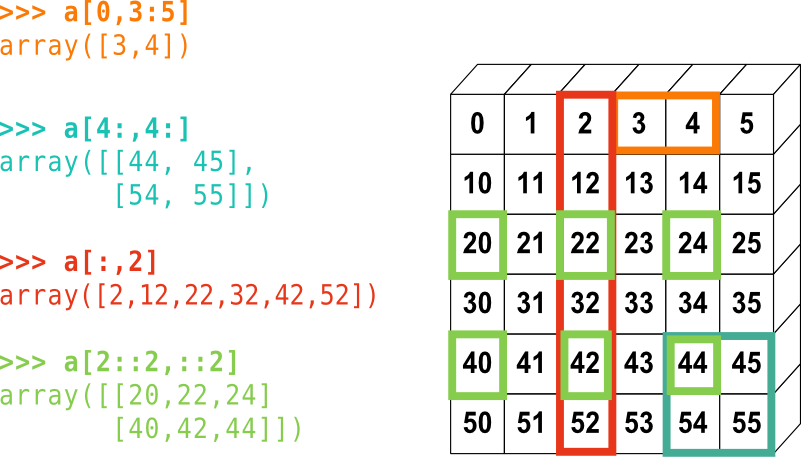
\includegraphics[scale=0.4]{img/numpy_slicing.png}
\centering
\caption{Graphical examples of numpy slicing.}\label{fig:4}
\end{figure}

This slicing does look really useful for cropping images. Doesn't it?

\subsection{Copies and Views}
A slicing operation creates a view on the original array, which is just a way of accessing array data. Thus the original array is not copied in memory. You can use np.may{\_}share{\_}memory() to check if two arrays share the same memory block. Note however, that this uses heuristics and may give you false positives. When modifying the view, the original array is modified as well:
\begin{lstlisting}
print "Explicit copy of a numpy array:"
a = np.arange(10)
b = a[::2].copy()
print "a = np.arange(10) and b = a[::2].copy().Do they share memory? %(bool)s.\n" % {"bool" : np.may{\_}share{\_}memory(a, b) }
\end{lstlisting}
If you want to force the copy of an array:
\begin{lstlisting}
print "Explicit copy of a numpy array:"
a = np.arange(10)
b = a[::2].copy()
print "a = np.arange(10) and b = a[::2].copy().Do they share memory? %(bool)s.\n" % {"bool" : np.may{\_}share{\_}memory(a, b) }
\end{lstlisting}
\subsection{Fancy indexing}
Numpy arrays can be indexed with slices, but also with boolean or integer arrays (masks). This method is called fancy indexing. Let me say that fancy indexing is really fancy. Differently from slicing it creates copies not views.
\begin{lstlisting}
print "Fancy indexing:"
np.random.seed(3)
a = np.random.random_integers(0, 20, 15)
mask = (a % 3 == 0)
print "a = %(a)s" % {"a":a}
print "The mask contains whether the value of an item is multiple of 3 or not. mask = (a % 3 == 0) = %(mask)s" % {"mask":mask}
print "a[mask] = %(a_masked)s.\n" % {"a_masked":a[mask]}
\end{lstlisting}
This looks real fun if you have to mask an image or if you want to extract values from a ROI (Region of Interest). Doesn't it?

You can perform fancy indexing also using python lists of integer indeces:
\begin{lstlisting}
print "Fancy indexing with integers arrays:"
a = np.arange(0, 100, 10)
print "a = np.arange(0, 100, 10) and a[[2, 3, 2, 4, 2]] = %(a_indexed)s" % {"a_indexed" : a[[2, 3, 2, 4, 2]]}
\end{lstlisting}
\begin{figure}[h]
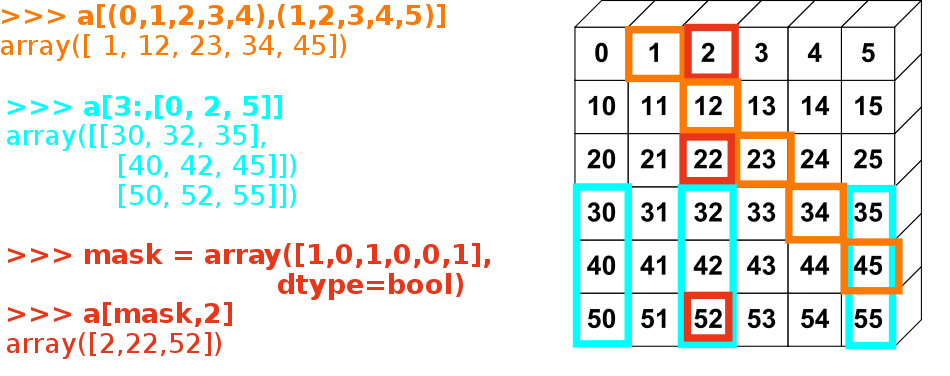
\includegraphics[scale=0.4]{img/numpy_fancy_indexing.png}
\centering
\caption{Graphical examples of numpy fancy indexing.}\label{fig:5}
\end{figure}
\subsection{Numpy for Matlab users}
You have been guided through the first steps of numpy and matplotlib libraries, however the things that you can do with those library are much more. In fact, in this tutorial important aspects such as array arithmetical operations, array broadcasting, reshaping and resizing are omitted. However, starting from this basic knowledge and the online documentations I am sure you can get really far very fast. For those of you that are use to Matlab and feel lazy about study new technologies, I would suggest to take a look at this address: \href{http://mathesaurus.sourceforge.net/matlab-numpy.html}{http://mathesaurus.sourceforge.net/matlab-numpy.html}. It contains all the most common Matlab functions translated to the correspondent numpy method. At this web address \href{http://conference.scipy.org/scipy2013/tutorials.php}{http://conference.scipy.org/scipy2013/tutorials.php} you can find some really interesting and high quality tutorials, where you can improve your knowledge of the libraries. 

\section{Exercises}
\subsection{Exercise 1}
Do you like pop art? What about to make your facebook profile picture Andy Warhol style? In this exercise you will have to take a RGB color picture, preferably a your profile picture, and create a Andy Warhol collage as in fig.7.

You may find useful OpenCV python bindings module (cv2), the OpenCV functions imread, cvtColor and merge. Then, you may find useful also the numpy functions hstack, vstack and astype.

Have fun!

\begin{figure}[h]
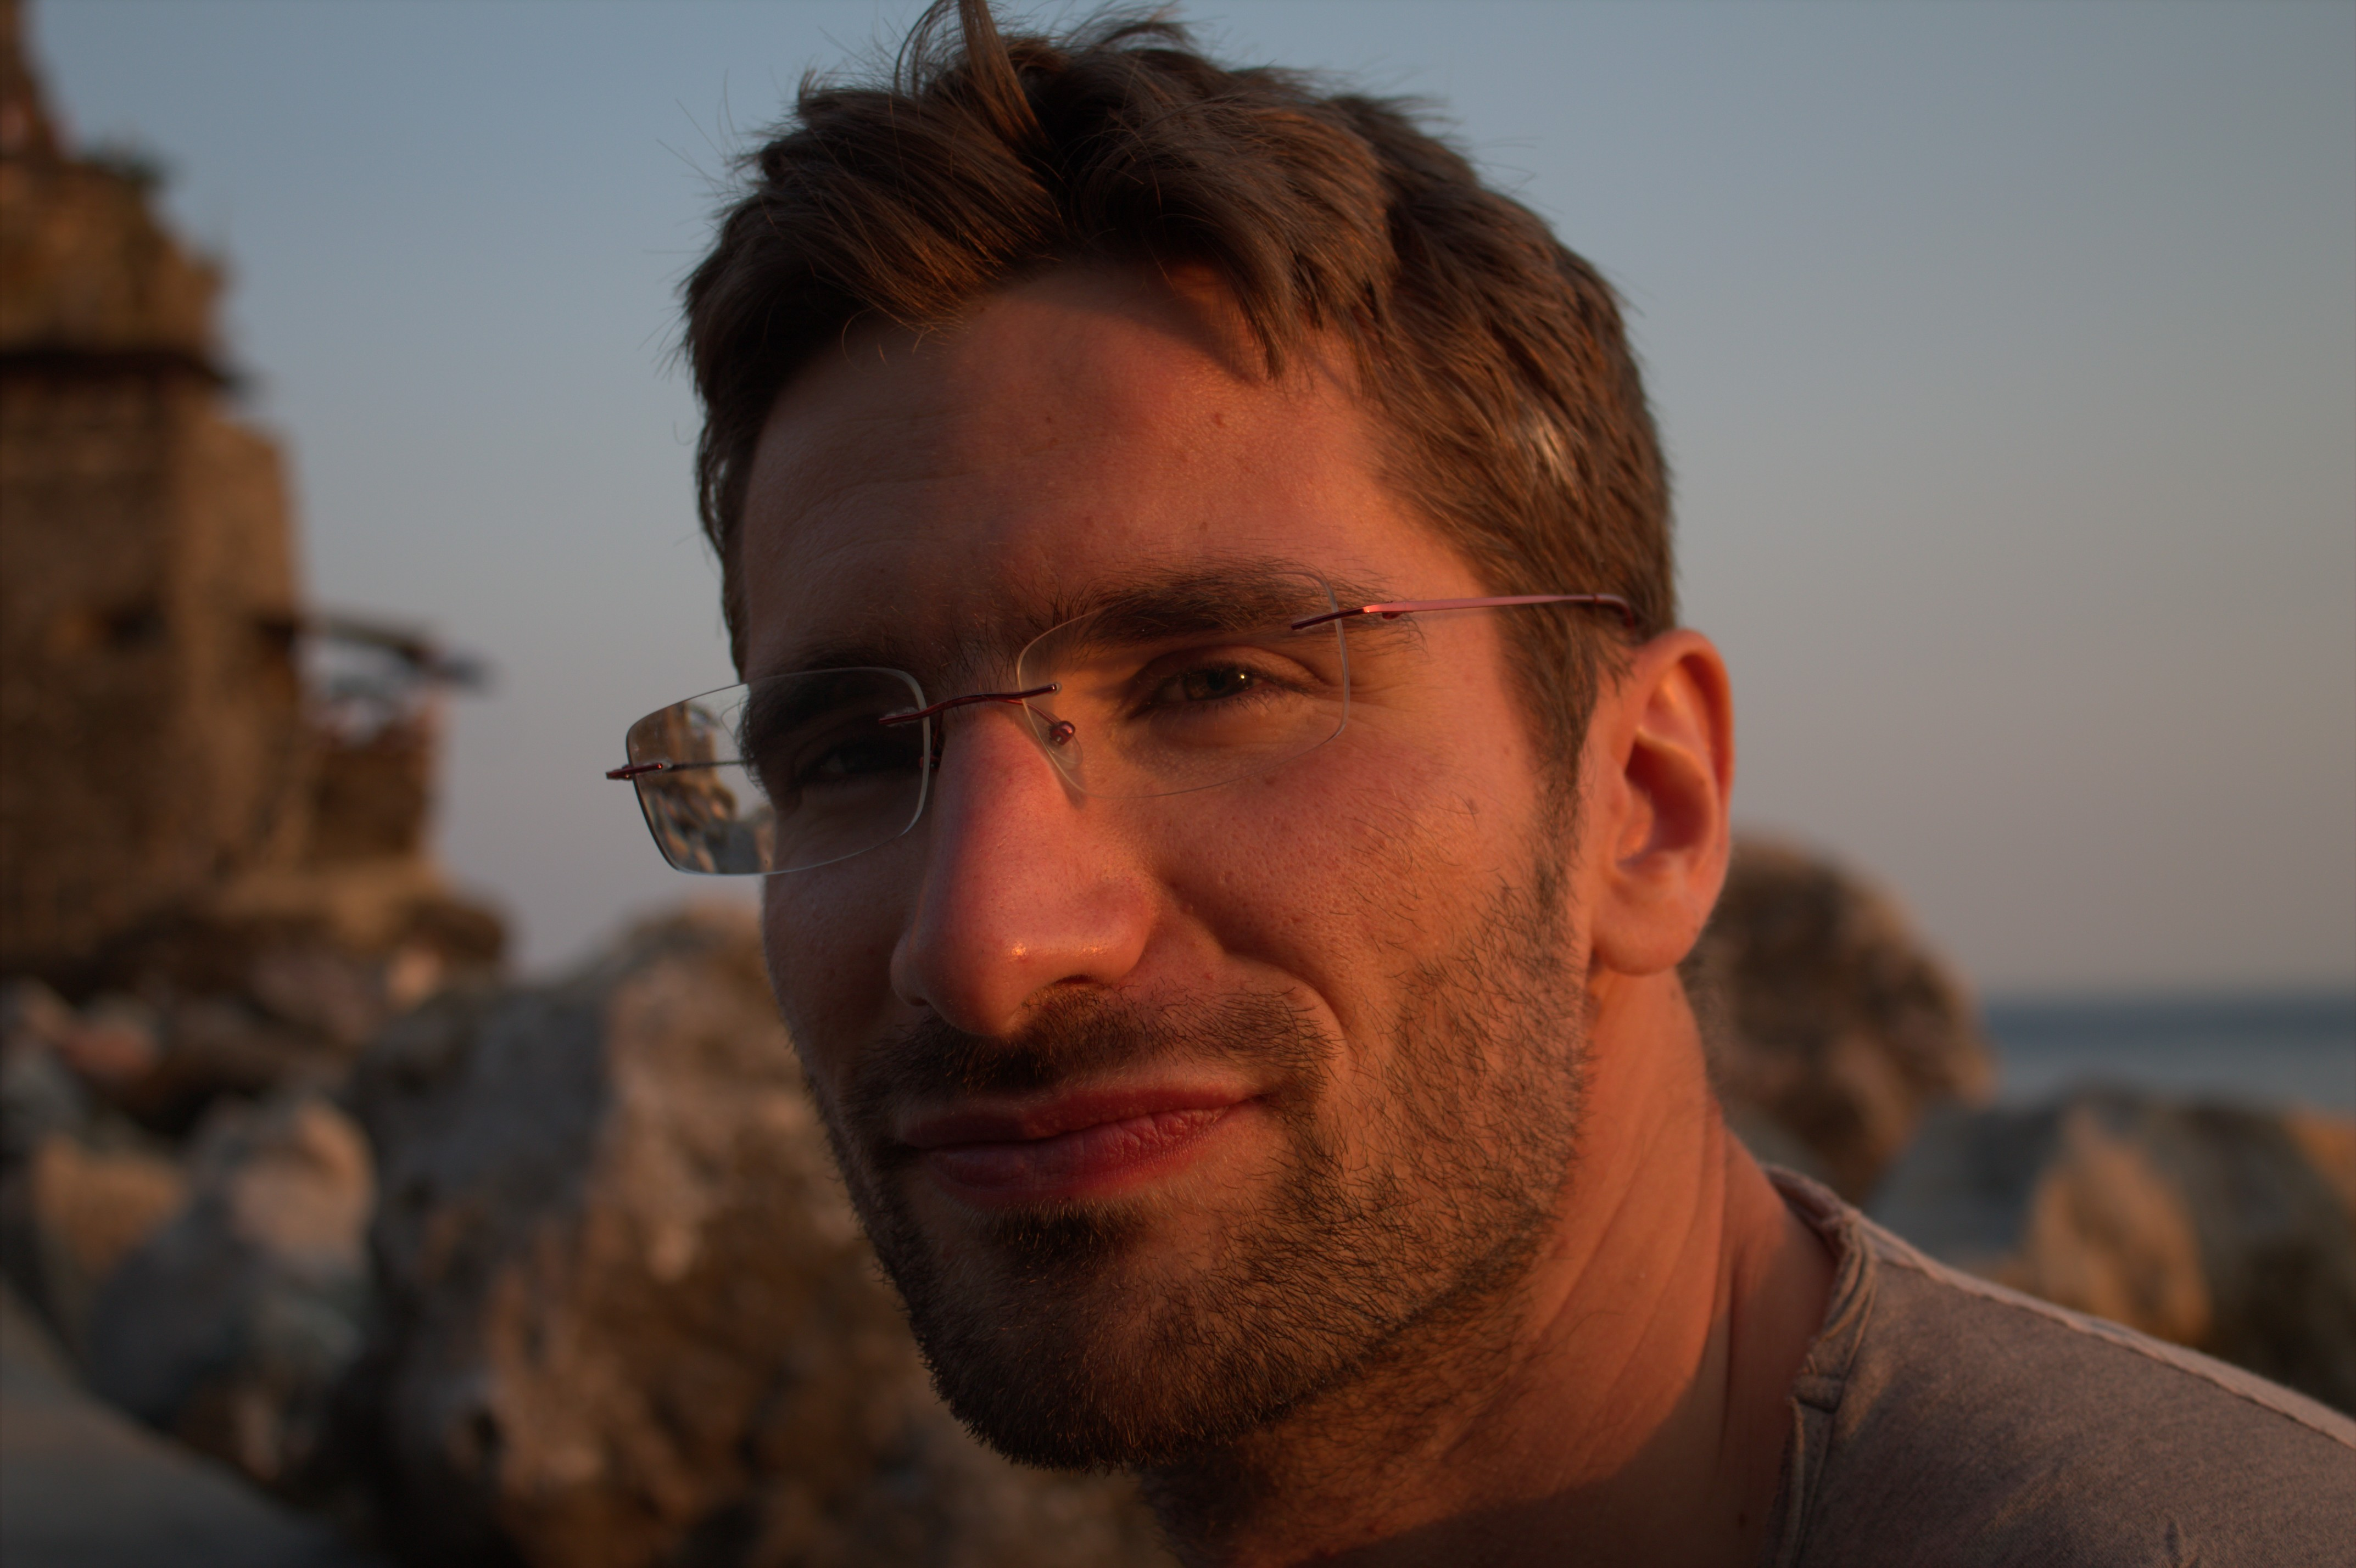
\includegraphics[width=0.5\textwidth]{img/profile.jpg}
\centering
\caption{My profile picture.}\label{fig:6}
\end{figure}
\begin{figure}[h]
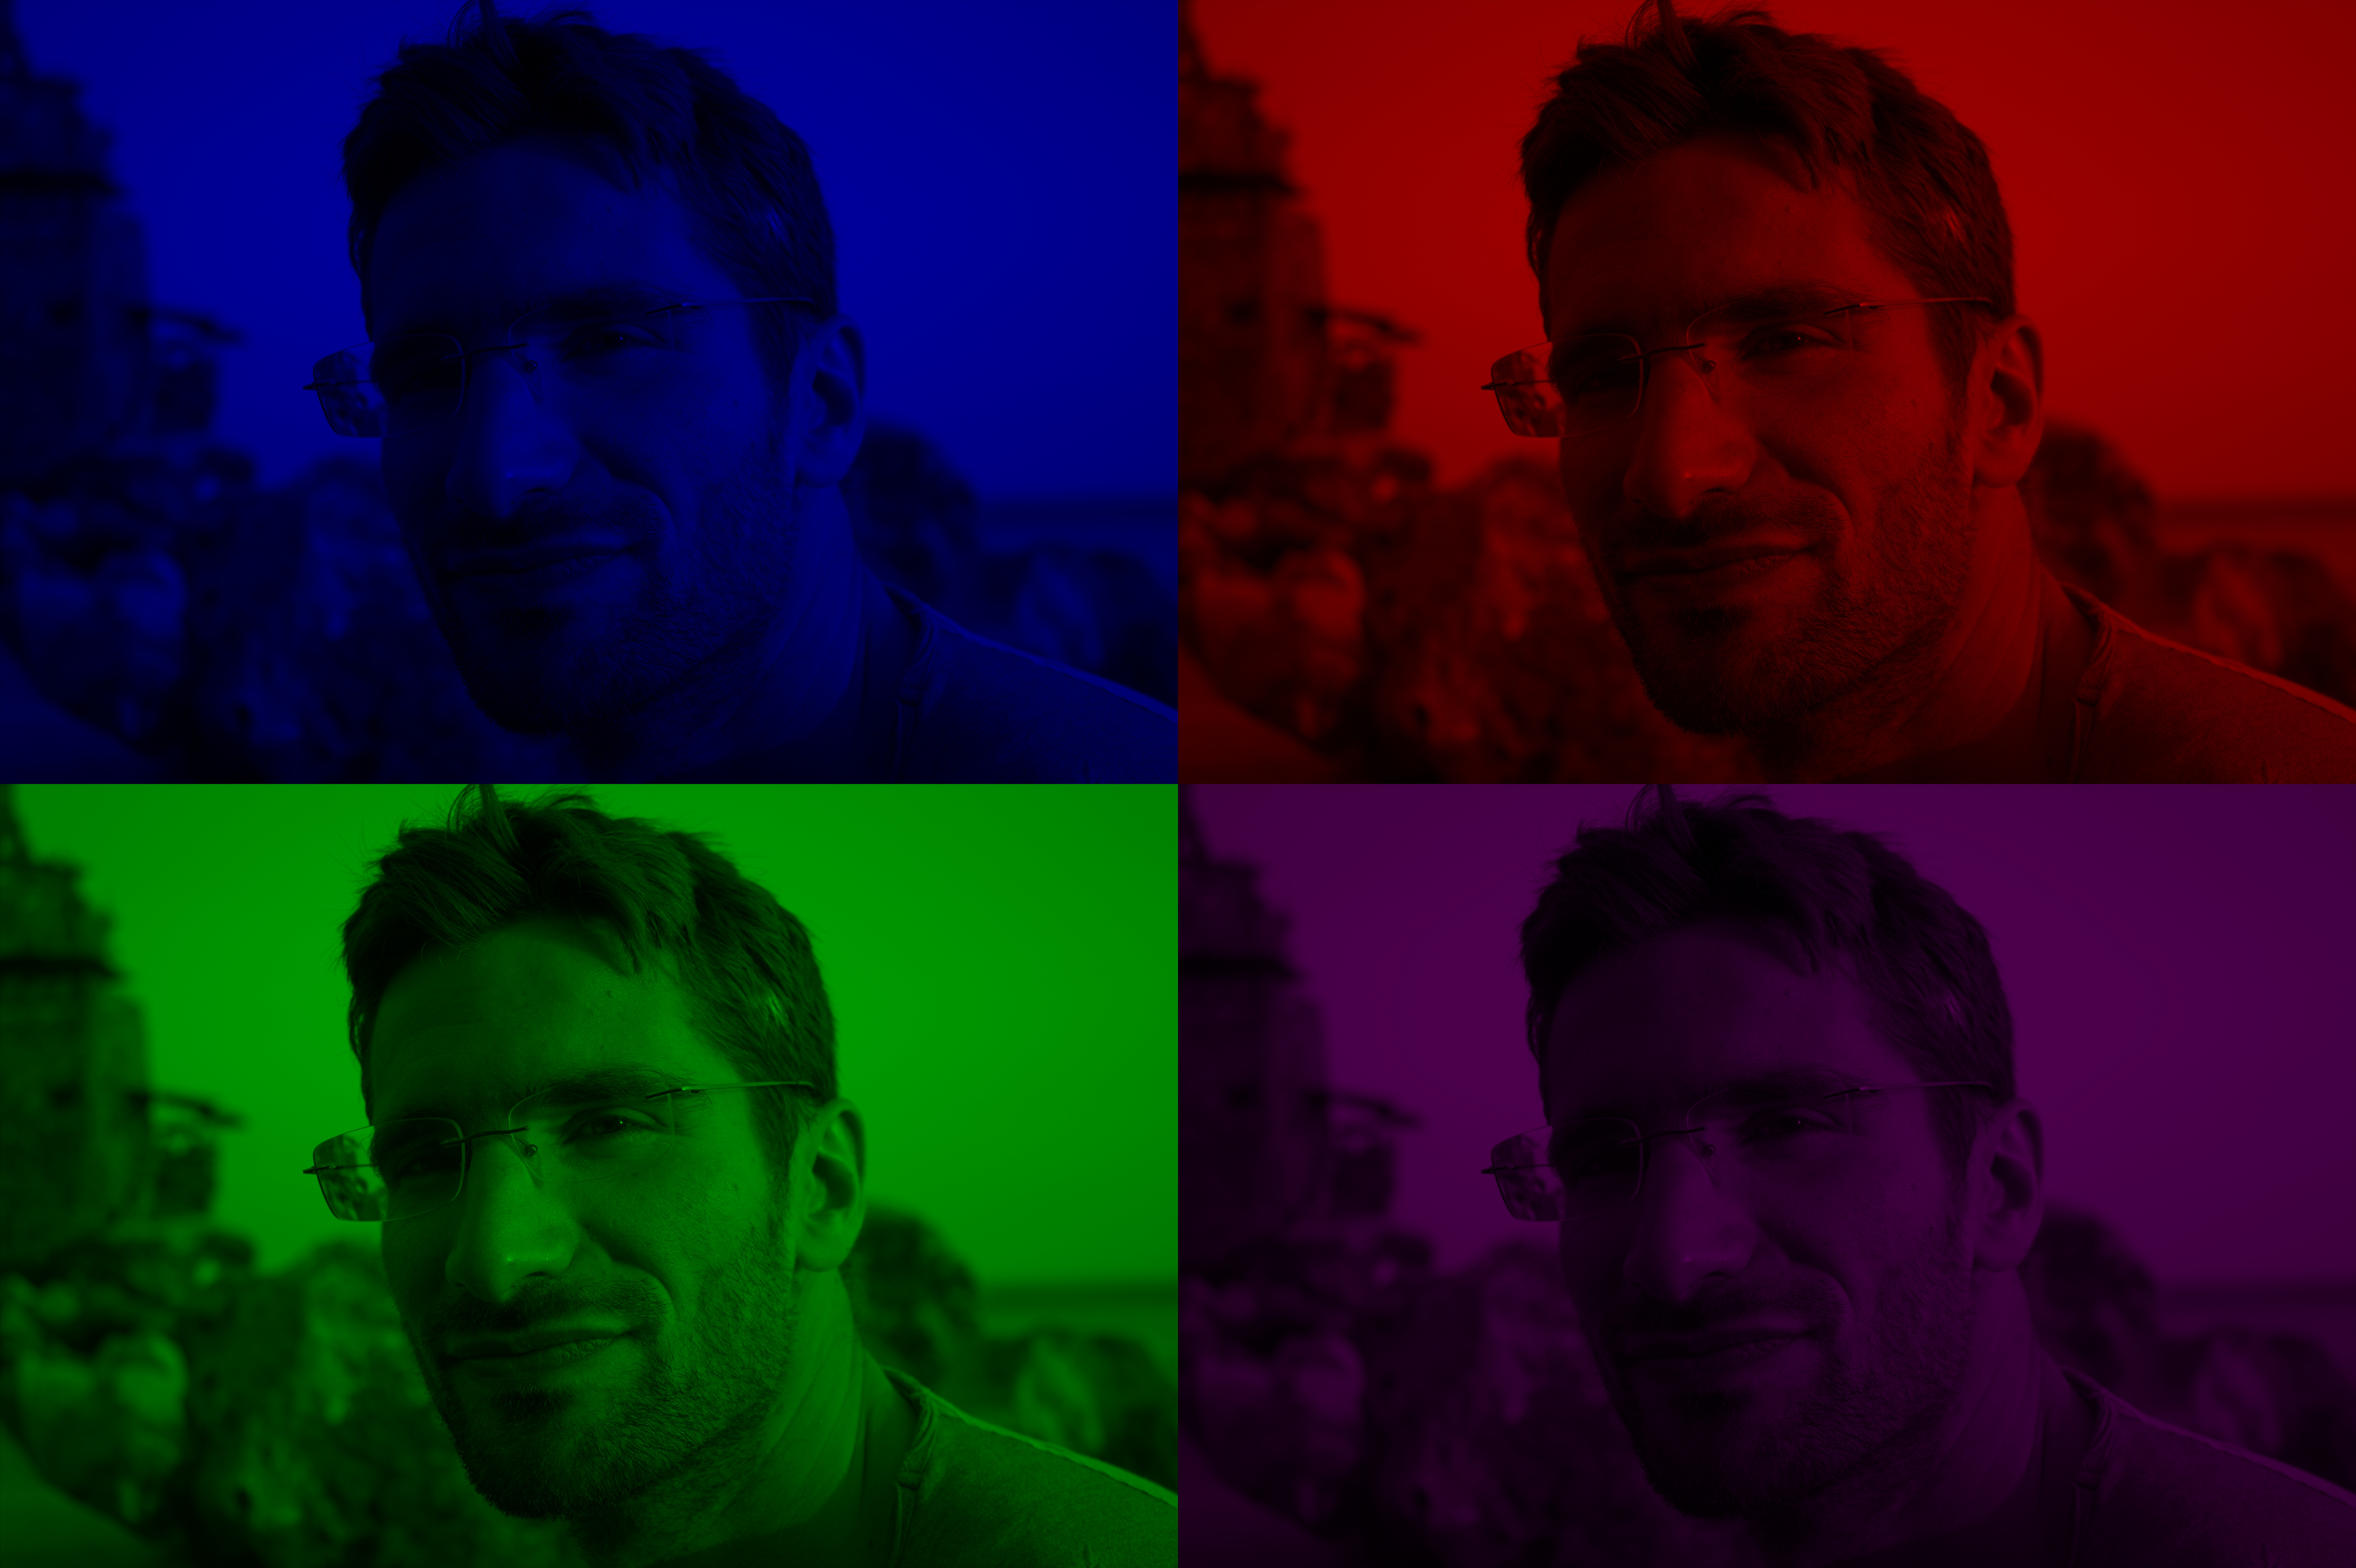
\includegraphics[width=0.5\textwidth]{img/new_profile.jpg}
\centering
\caption{My profile picture Andy Warhol style.}\label{fig:7}
\end{figure}

\subsection{Exercise 2}
Threshold the coins image and set to black the foreground, as in fig.9.

Enjoy!

\begin{figure}[h]
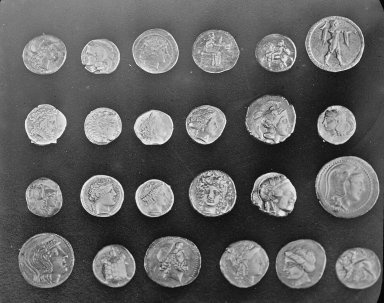
\includegraphics[width=0.5\textwidth]{img/coins.jpg}
\centering
\caption{Coins pictures.}\label{fig:8}
\end{figure}

\begin{figure}[h]
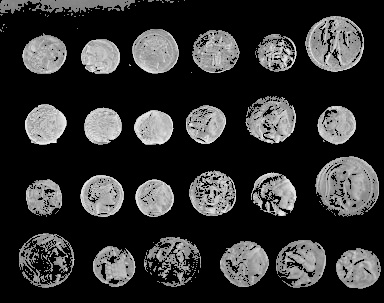
\includegraphics[width=0.5\textwidth]{img/new_coins.jpg}
\centering
\caption{Coins pictures with foreground to black.}\label{fig:9}
\end{figure}

\begin{figure}[h]
\centering
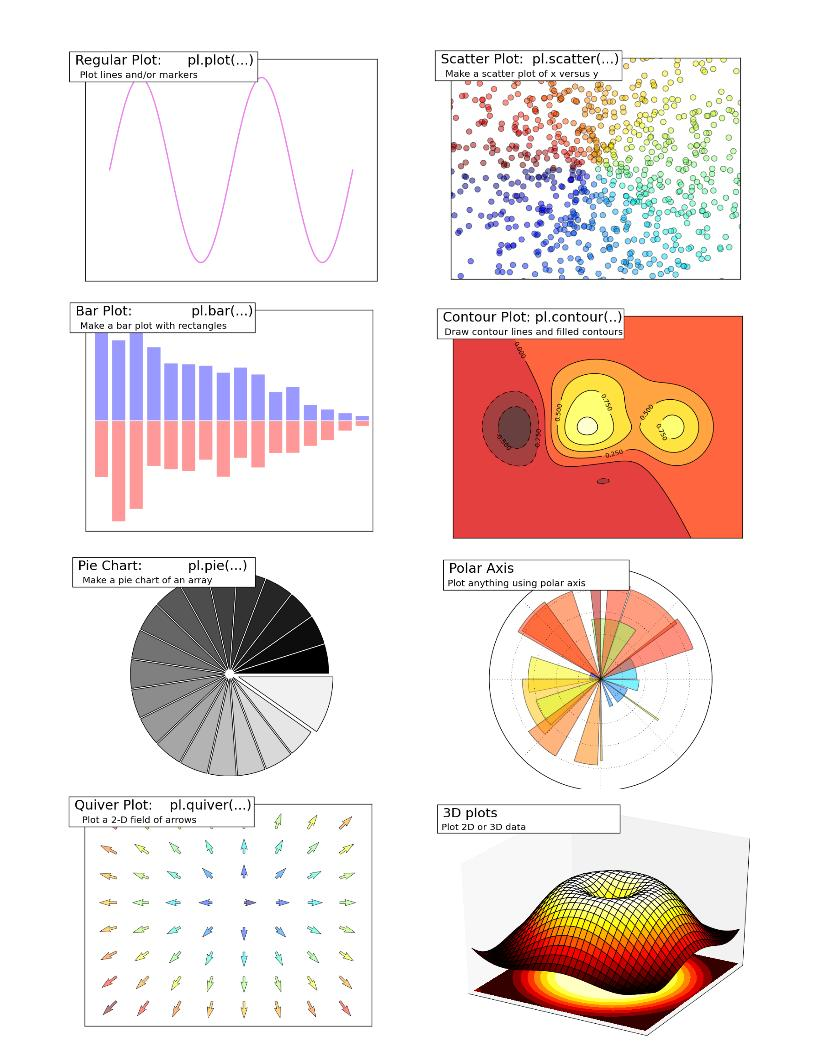
\includegraphics[width=1.0\textwidth]{img/matplotlib_all.jpg}
\caption{Matplotlib plotting methods.}\label{fig:3}
\end{figure}

\end{document}